\subsection{エンコーダ誤差とスリップによるセンサ追加の必要性}

直前までのオドメトリでは、左右の車輪エンコーダから得た回転量を地面上の移動量へ変換し、差動二輪ロボットの位置と方位角を逐次積分した。左右車輪の半径を $r_L,r_R$ [m]、車輪間距離を $b$ [m]、時刻 $k$ の短い区間における車輪角の増分を $\Delta\phi_{L,k},\Delta\phi_{R,k}$ [rad] とすると、すべりがなく、半径が正しく、パルス数が十分細かいという条件では
\begin{align}
  \Delta s_{L,k}&=r_L\Delta\phi_{L,k},&
  \Delta s_{R,k}&=r_R\Delta\phi_{R,k},\\
  \Delta s_k&=\frac{\Delta s_{R,k}+\Delta s_{L,k}}{2},&
  \Delta\theta_k&=\frac{\Delta s_{R,k}-\Delta s_{L,k}}{b}
\end{align}
で進む。ここで $\Delta s_{L,k},\Delta s_{R,k},\Delta s_k$ は [m]、$\Delta\theta_k$ は [rad] である。この式は、車輪の回転量と地面上の移動量が一対一に対応するという機械的な仮定を含んでいる。次に必要になるのは、この仮定がどの程度の速さで破れるかを数値で見ることである。

まず車輪半径の設定誤差を考える。オドメトリが使う半径を
\begin{equation}
  \hat{r}_i=(1+\epsilon_i)r_i,\qquad i\in\{L,R\}
\end{equation}
と書くと、推定された車輪移動量は
\begin{equation}
  \hat{\Delta s}_{i,k}
  =
  \hat{r}_i\Delta\phi_{i,k}
  =
  (1+\epsilon_i)\Delta s_{i,k}
\end{equation}
である。したがって、半径誤差だけによる方位角増分のずれは
\begin{equation}
  \hat{\Delta\theta}_k-\Delta\theta_k
  =
  \frac{\epsilon_R\Delta s_{R,k}-\epsilon_L\Delta s_{L,k}}{b}
\end{equation}
となる。左右が同じ割合でずれると主に距離の尺度が変わり、左右差をもつと方位角が少しずつ曲がる。たとえば $b=0.32\,\mathrm{m}$ のロボットで、右車輪だけが $1.0\,\%$ 大きく見積もられ、左右とも地面上で $2.00\,\mathrm{m}$ 進んだ場合、右車輪距離の過大評価は $0.020\,\mathrm{m}$ であり、方位角のずれは
\begin{equation}
  \frac{0.020}{0.32}=0.0625\,\mathrm{rad}
  \simeq 3.58^\circ
\end{equation}
になる。半径誤差は小さく見えても、走行距離に比例して蓄積する。

次に、パルス量子化を入れる。1 回転あたりのエンコーダ分解能を $N$ [count/rev] とすると、1 count が表す車輪外周上の距離は
\begin{equation}
  q=\frac{2\pi r}{N}\quad[\mathrm{m/count}]
\end{equation}
である。$r=0.050\,\mathrm{m}$、$N=360\,\mathrm{count/rev}$ なら
\begin{equation}
  q
  =
  \frac{2\pi\cdot0.050}{360}
  =
  8.73\times10^{-4}\,\mathrm{m/count}
  =
  0.873\,\mathrm{mm/count}
\end{equation}
である。累積 count を整数に丸めて読むと、各車輪の距離換算残差は高々約 $q/2=0.436\,\mathrm{mm}$ である。左右の丸め残差が反対符号になった瞬間の方位角残差は、おおまかに
\begin{equation}
  \abs{\delta\theta_q}
  \le
  \frac{q}{b}
  =
  \frac{0.873\times10^{-3}}{0.32}
  =
  2.73\times10^{-3}\,\mathrm{rad}
  \simeq0.156^\circ
\end{equation}
である。量子化は 1 回の読み取りでは小さいが、低速時には速度推定を階段状にし、微小な旋回や停止直前の判定を粗くする。

最後に、短いスリップ区間を入れる。左車輪が回転した外周距離を $r_L\Delta\phi_{L,k}$ とし、地面に実際に伝わった割合を $\lambda_{L,k}\in[0,1]$ と書くと、
\begin{equation}
  \Delta s^{\mathrm{ground}}_{L,k}
  =
  \lambda_{L,k}r_L\Delta\phi_{L,k}
\end{equation}
である。エンコーダは車輪軸の回転を測るので、$\lambda_{L,k}$ を直接測っていない。左車輪だけがすべった区間では、エンコーダが使う距離と地面上の距離の差
\begin{equation}
  \Delta s_{\mathrm{loss},k}
  =
  (1-\lambda_{L,k})r_L\Delta\phi_{L,k}
\end{equation}
が残り、真の旋回増分とエンコーダ由来の旋回増分の差は近似的に
\begin{equation}
  \Delta\theta_{\mathrm{true},k}
  -
  \Delta\theta_{\mathrm{enc},k}
  \simeq
  \frac{\Delta s_{\mathrm{loss},k}}{b}
\end{equation}
となる。半径誤差や量子化はエンコーダ値の換算に現れるが、スリップは「車輪は回ったが、機体は同じだけ進まなかった」という地面との相互作用に現れる。

図\ref{fig:flow6-encoder-slip-examples}は、$b=0.32\,\mathrm{m}$、$r=0.050\,\mathrm{m}$、$N=360\,\mathrm{count/rev}$ の差動二輪ロボットを 8 s 走らせた計算例である。$3.20$ s から $3.80$ s まで左車輪だけがすべり、車輪が回した距離の $60\,\%$ だけが地面へ伝わるとした。通常のエンコーダオドメトリは count から進んだつもりの経路を積分するため、すべり区間のあとも真の経路から離れたままになる。さらに、左半径を $+1.5\,\%$、右半径を $-1.0\,\%$ だけ誤って換算すると、方位角のずれが同じ方向に重なり、8 s 後の位置誤差は $0.390\,\mathrm{m}$ から $0.676\,\mathrm{m}$ へ増える。方位角誤差も $-14.53^\circ$ から $-26.96^\circ$ へ広がる。

\begin{figure}[tb]
\centering
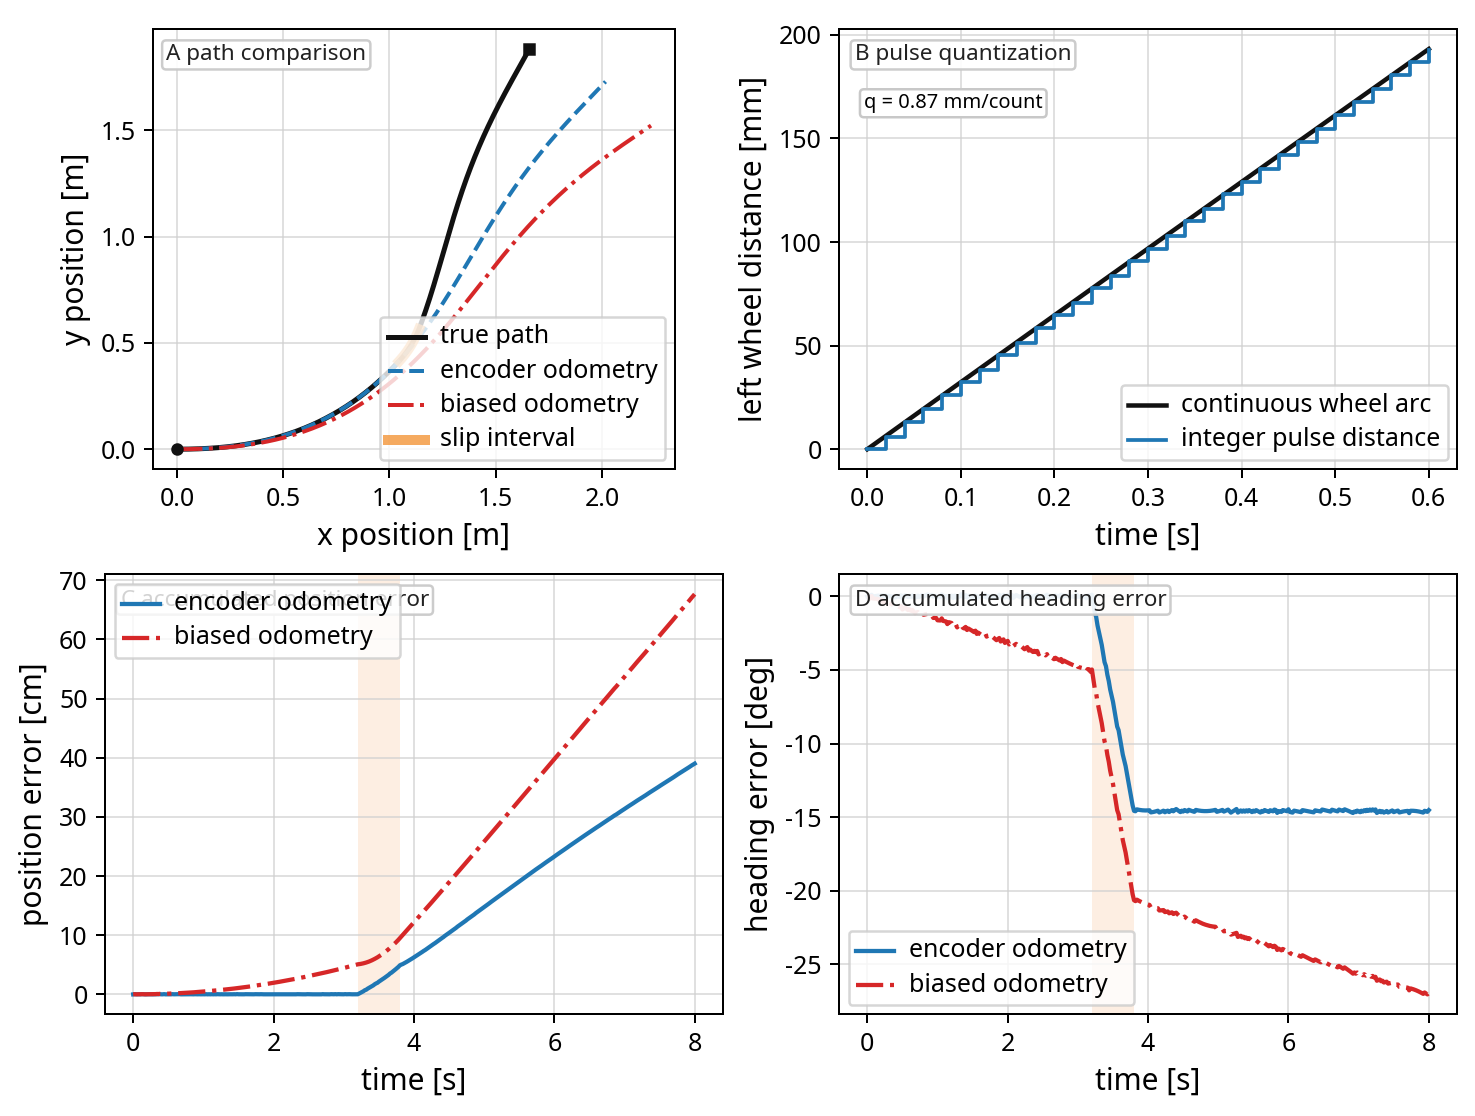
\includegraphics[width=0.95\linewidth,bb=0 0 1476 1116]{figures/flow6_encoder_slip_examples.png}
\caption{差動二輪ロボットにおける真の経路、通常のエンコーダオドメトリ、半径誤差を重ねたオドメトリの比較。左車輪は $3.20$--$3.80\,\mathrm{s}$ だけすべり、車輪外周の移動量 $0.204\,\mathrm{m}$ のうち $0.081\,\mathrm{m}$ が地面上の移動に変換されない。量子化の 1 count は $0.873\,\mathrm{mm}$ であり、短時間の距離推定を階段状にする。}
\label{fig:flow6-encoder-slip-examples}
\end{figure}

\begin{table}[tb]
\centering
\footnotesize
\setlength{\tabcolsep}{3pt}
\begin{tabular}{>{\raggedright\arraybackslash}p{0.20\linewidth}>{\raggedright\arraybackslash}p{0.25\linewidth}>{\raggedright\arraybackslash}p{0.23\linewidth}>{\raggedright\arraybackslash}p{0.22\linewidth}}
\hline
要因 & 代表値 & 距離への影響 & 方位角への影響\\
\hline
半径設定ずれ & 右だけ $+1.0\,\%$, $s=2.00\,\mathrm{m}$ & $+20\,\mathrm{mm}$ & $0.020/0.32=3.58^\circ$\\
パルス量子化 & $q=0.873\,\mathrm{mm/count}$ & $\le0.436\,\mathrm{mm}$ & $\le0.156^\circ$\\
左車輪スリップ & $\lambda=0.60$, 回転距離 $0.204\,\mathrm{m}$ & 損失 $0.081\,\mathrm{m}$ & $0.081/0.32=14.6^\circ$\\
\hline
\end{tabular}
\caption{半径誤差、パルス量子化、短時間スリップが距離と方位角へ与える代表的な大きさ。スリップは短時間でも方位角に大きく効き、しかもエンコーダ count だけでは検出できない。}
\label{tab:flow6-encoder-error-contributions}
\end{table}

表\ref{tab:flow6-encoder-error-contributions}の値は、エンコーダだけで自己位置を閉じると何が失われるかを分けている。半径誤差は、同じ count を何 m と読むかの尺度誤差である。量子化は、連続的な車輪角を整数 count に丸めることによる読み取り誤差である。スリップはこれらと性質が異なり、count 列そのものは正常に見えているのに、地面上の移動量が同じでなくなる。エンコーダ値だけを入力にして
\begin{equation}
  (x_k,y_k,\theta_k)
  =
  F\left((x_{k-1},y_{k-1},\theta_{k-1}),\Delta n_{L,k},\Delta n_{R,k}\right)
\end{equation}
と積分している限り、同じ $\Delta n_{L,k},\Delta n_{R,k}$ から「車輪が地面を押して進んだ場合」と「車輪が空転気味に回った場合」を区別できない。方位角についても同じで、左右 count の差から積分した $\theta$ がゆっくりずれても、エンコーダだけでは外部基準に対する方位角の残差を作れない。

この不可観測なずれが、次に慣性センサを加える理由である。IMU は車輪の回転ではなく、機体に取り付けたセンサとして角速度や加速度に対応する信号を出す。もちろん IMU にもバイアス、ノイズ、重力方向との混同があるため、単体で完全な位置を与えるわけではない。それでも、車輪 count と独立した方位角変化の手掛かりを持つため、スリップや方位角ドリフトを検出・補正するための別の観測経路になる。次の段階では、IMU の式を急いで導入する前に、ジャイロ積分、加速度計が見る重力、バイアスとノイズの蓄積を順に調べ、エンコーダだけでは閉じなかった残差をどの信号で見るのかを明確にする。
